\documentclass[oneside,12pt,letterpaper]{article}

% Imports and Definitions
%% Packages
\usepackage{amsmath}
\usepackage{amsfonts}
\usepackage{amssymb}
\usepackage{amsthm}
\usepackage{arydshln}
\usepackage{color}
\usepackage{extramarks}
\usepackage{fancyhdr}
\usepackage{float}
\usepackage[margin=1in]{geometry}
\usepackage{graphicx}
\usepackage{listings}
\usepackage{multicol}
\usepackage{setspace}
\usepackage{subcaption}
\usepackage{textcomp}
\usepackage{url}
\usepackage{xspace}
\usepackage{mathtools}

%% Commands
%%% Metadata
\newcommand{\metaTitle}{Comprehensive Exam}
\newcommand{\metaDueDate}{November 24, 2020}
\newcommand{\metaDueTime}{04:00 PM}
\newcommand{\metaSchool}{IUPUI}
\newcommand{\metaClass}{STAT 52400}
\newcommand{\metaDepartment}{Statistics Department}
\newcommand{\metaAuthorName}{Ross Grinvalds}

%%% Aliases
\newcommand{\Bias}{\mathrm{Bias}}
\newcommand{\Cov}{\mathrm{Cov}}
\newcommand{\dd}[1]{\frac{\mathrm{d}}{\mathrm{d}x} (#1)}
\newcommand{\dx}{\mathrm{d}x}
\newcommand{\E}{\mathrm{E}}
\newcommand{\m}[1]{\begin{bmatrix*}[r]#1\end{bmatrix*}}
\newcommand{\md}[1]{\begin{vmatrix*}#1\end{vmatrix*}}
\newcommand{\mf}[1]{\mathrm{\bf{#1}}}
\newcommand{\p}[1]{\begin{pmatrix}#1\end{pmatrix}} 
\newcommand{\pdd}[2]{\frac{\partial}{\partial #1} (#2)}
\newcommand{\solution}{\textbf{\large Solution}}
\newcommand{\T}{\intercal}
\newcommand{\Var}{\mathrm{Var}}

%%% Math Functions
\makeatletter
\newsavebox{\mybox}\newsavebox{\mysim}
\newcommand{\distras}[1]{%
  \savebox{\mybox}{\hbox{\kern3pt$\scriptstyle#1$\kern3pt}}%
  \savebox{\mysim}{\hbox{$\sim$}}%
  \mathbin{\overset{#1}{\kern\z@\resizebox{\wd\mybox}{\ht\mysim}{$\sim$}}}%
}
\makeatother

\newcommand{\indep}{\perp \!\!\! \perp}

%% Environments
%%% R Code
\newcommand{\ri}[1]{\lstinline{#1}}  %% Short for 'R inline'

\lstnewenvironment{rc}[1][]{
	\lstset{commentstyle=\color{red}, keywordstyle=\color{black}, showstringspaces=true, language=R, basicstyle=\ttfamily\tiny}
}{}
\lstset{language=R}


% Settings
%% Document-wide
\pagestyle{fancy}

%% Header and Footer
\setlength{\headheight}{15pt}
\lhead{\metaAuthorName}
\chead{\metaSchool\ \metaClass:\ \metaTitle}
\rhead{\metaDepartment}
\cfoot{\thepage}

%% Title Page
\title{
	\vspace{1in}
	\textmd{\textbf{\metaSchool\ \metaClass:\ \metaTitle}}\\
	\normalsize\vspace{0.1in}\small{Due\ by\ \metaDueDate\ at \metaDueTime}\\
	\vspace{6in}
}
\author{\metaAuthorName}
\date{}


\begin{document}
\maketitle

\section*{Problem 4.28}
The air pollution data from Table 1.5 was imported into R using the `tidyverse` library. This question focuses on a univariate normality assessment of the solar radiation measurements contained in the dataset. The quantile-quantile plot is shown below. The plot demonstrates a deviation in the left tail of the distribution from normality. This suggests that solar radiation may not be normally distributed.
\begin{center}
	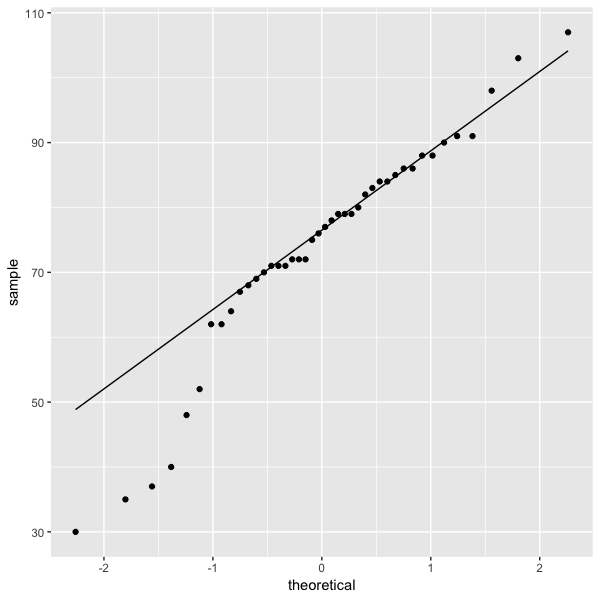
\includegraphics[width=4in]{plot_4_28_qq.png}
\end{center}
A formal test for the normality of this variable can be conducted via a normal quantile statistic. The statistic is defined as follows: $$r_Q = \frac{\sum_{j = 1}^{40} \p{x_{(j)} - \bar{x}} \p{q_{(j)} - \bar{q}}}{\sqrt{\sum_{j = 1}^{40} \p{x_{(j)} - \bar{x}}^2} \sqrt{\sum_{j = 1}^{40} \p{q_{(j)} - \bar{q}}^2}} = \frac{SS_{xq}}{\sqrt{SS_x} \sqrt{SS_q}}$$ The requisite quantities were computed in R as $SS_{xq} = 686.8434$, $SS_x = 12321.14$, and $SS_q = 40.74975$. The resulting test statistic is $r_Q = 0.9693258$. Using the critical values from table 4.2 in Johnson and Wichern, the assumption of normality of solar radiation should be rejected if $r_Q < 0.9726$ for sample size $n = 40$ and confidence level $\alpha = 0.05$ (181). Therefore, the null hypothesis should be rejected. That is, the evidence suggests the data is not normally distributed.

\newpage
\section*{Problem 4.29}
This problem provides further analysis on the air pollution data from Table 1.5, now from a bivariate perspective on two of the selected variables, $X_1 = NO_2$ and $X_2 = O_3$, from the dataset. Prior to a bivariate analysis, a simpler univariate analysis will help to identify much simpler problems. A suite of tests was performed on $X_1$ and $X_2$. 
\\
\\For $X_1$, first a histogram of the data helps provide an understanding of the univariate spread. In this case, it is clear the the data is moderately right-skewed and not symmetrically distributed. A quantile-quantile plot also suggests the data may not be normally distributed. See Figure 1. Statistical tests including the Shapiro-Wilks and the correlation quantile test further suggest that the data is not normally distributed, as both tests imply that the null hypothesis (normally distributed data) should be rejected. The R output is included in Figure 2.
\begin{figure}[H]
\begin{subfigure}{.33\textwidth}
  \centering
  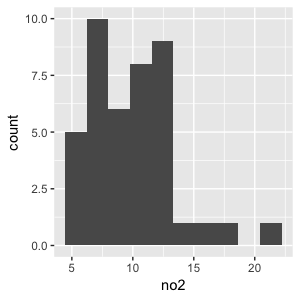
\includegraphics[width=.8\linewidth]{plot_4_29_X1hist.png}
  \caption{histogram}
  \label{fig:sfig1}
\end{subfigure}%
\begin{subfigure}{.33\textwidth}
  \centering
  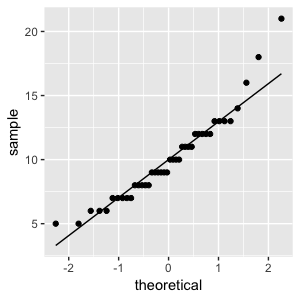
\includegraphics[width=.8\linewidth]{plot_4_29_X1qq.png}
  \caption{quantile-quantile plot}
  \label{fig:sfig2}
\end{subfigure}
\begin{subfigure}{.33\textwidth}
  \centering
  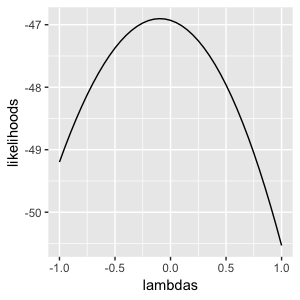
\includegraphics[width=.8\linewidth]{plot_4_29_X1bxcx.png}
  \caption{Box-Cox likelihood}
  \label{fig:sfig3}
\end{subfigure}%
\caption{Selected plots from the univariate analysis of $X_1$.} 
\end{figure}
\begin{figure}[H]
\begin{rc}
	Shapiro-Wilk normality test

data:  df[[var]]
W = 0.93004, p-value = 0.013


	Probability Plot Correlation Coefficient Test

data:  df[[var]]
ppcc = 0.96247, n = 42, p-value = 0.0121
alternative hypothesis: df[[var]] differs from a Normal distribution

# A tibble: 41 x 2
  lambdas likelihoods
    <dbl>       <dbl>
1  -0.100       -46.9
\end{rc}
\caption{Selected R output from the univariate analysis of $X_1$.}
\end{figure}
As a remedy for the nonnormality of the data, an ideal transformation was identified via the Box-Cox method. The maximum likelihood of an array of possible transformation values led to a selection of $\hat{\lambda} = -0.1$. The updated analysis suggests an improvement when compared to the data prior to the transformation.
\begin{figure}[H]
\begin{subfigure}{.5\textwidth}
  \centering
  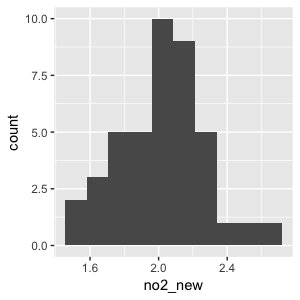
\includegraphics[width=.8\linewidth]{plot_4_29_X1newhist.png}
  \caption{histogram}
  \label{fig:sfig1}
\end{subfigure}%
\begin{subfigure}{.5\textwidth}
  \centering
  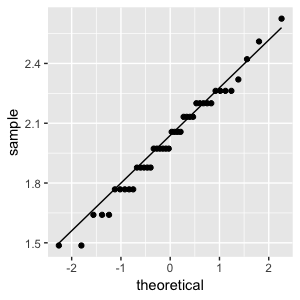
\includegraphics[width=.8\linewidth]{plot_4_29_X1newqq.png}
  \caption{quantile-quantile plot}
  \label{fig:sfig2}
\end{subfigure}
\caption{Updated plots after the transformation of $X_1$.}
\end{figure}
Similarly, a univariate analysis of $X_2$ was performed. The analysis was similar to that of $X_1$ in that the data appeared to be skewed right and exhibiting nonnormality. A Box-Cox transformation of the data was applied to the data using $\hat{\lambda} = 0.25$. Figures 4 - 6 demonstrate the same process as provided in the case for $X_1$.
\begin{figure}[H]
\begin{subfigure}{.33\textwidth}
  \centering
  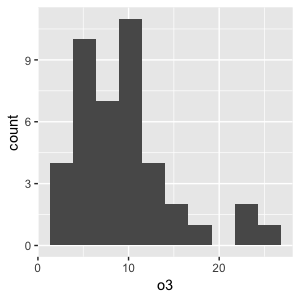
\includegraphics[width=.8\linewidth]{plot_4_29_X2hist.png}
  \caption{histogram}
  \label{fig:sfig1}
\end{subfigure}%
\begin{subfigure}{.33\textwidth}
  \centering
  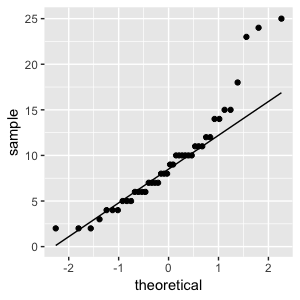
\includegraphics[width=.8\linewidth]{plot_4_29_X2qq.png}
  \caption{quantile-quantile plot}
  \label{fig:sfig2}
\end{subfigure}
\begin{subfigure}{.33\textwidth}
  \centering
  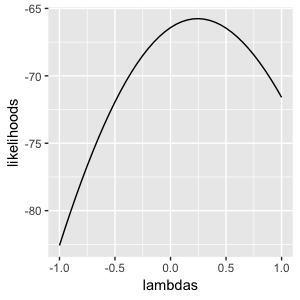
\includegraphics[width=.8\linewidth]{plot_4_29_X2bxcx.png}
  \caption{Box-Cox likelihood}
  \label{fig:sfig3}
\end{subfigure}%
\caption{Selected plots from the univariate analysis of $X_2$.} 
\end{figure}
\begin{figure}[H]
\begin{rc}
	Shapiro-Wilk normality test

data:  df[[var]]
W = 0.89603, p-value = 0.001098


	Probability Plot Correlation Coefficient Test

data:  df[[var]]
ppcc = 0.94754, n = 42, p-value = 0.0018
alternative hypothesis: df[[var]] differs from a Normal distribution

# A tibble: 41 x 2
  lambdas likelihoods
    <dbl>       <dbl>
1    0.25       -65.8
\end{rc}
\caption{Selected R output from the univariate analysis of $X_2$.}
\end{figure}
\begin{figure}[H]
\begin{subfigure}{.5\textwidth}
  \centering
  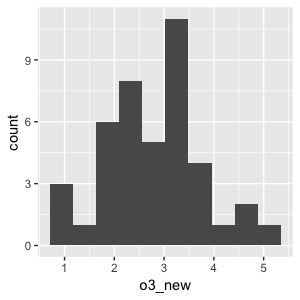
\includegraphics[width=.8\linewidth]{plot_4_29_X2newhist.png}
  \caption{histogram}
  \label{fig:sfig1}
\end{subfigure}%
\begin{subfigure}{.5\textwidth}
  \centering
  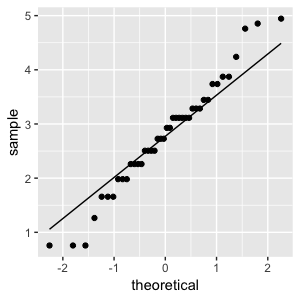
\includegraphics[width=.8\linewidth]{plot_4_29_X2newqq.png}
  \caption{quantile-quantile plot}
  \label{fig:sfig2}
\end{subfigure}
\caption{Updated plots after the transformation of $X_2$.}
\end{figure}
Overall, the spread of the data seems to have greatly improved. This is evident by observing the scatter of the points of $X_1$ against those of $X_2$, as shown in Figure 7. The overall shape of the spread should be ellipsoidal.
\begin{figure}[H]
\begin{subfigure}{.5\textwidth}
  \centering
  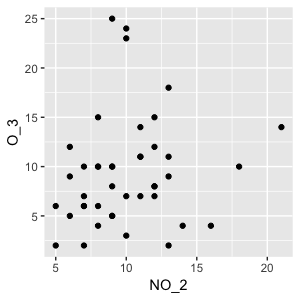
\includegraphics[width=.8\linewidth]{plot_4_29_X1X2scatter.png}
  \caption{before transformation}
  \label{fig:sfig1}
\end{subfigure}%
\begin{subfigure}{.5\textwidth}
  \centering
  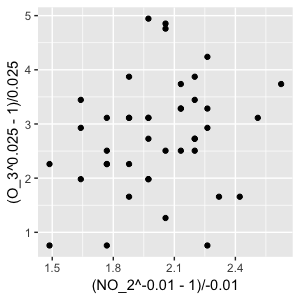
\includegraphics[width=.8\linewidth]{plot_4_29_X1X2newscatter.png}
  \caption{after transformation}
  \label{fig:sfig2}
\end{subfigure}
\caption{Bivariate scatter plots before and after transformation of the univariate distributions.}
\end{figure}

\begin{enumerate}
	\item[\bf{a)}] The squared statistical distances from the sample mean vector were computed for both the untransformed and the transformed data using matrix operations in R. Using a cutoff of $0.98$, the quantile of a chi-squared distribution on two degrees of freedom is $\mathcal{X}_2^2(0.98)=7.824$. Given this information, even in the untransformed data, there are only two points that exhibit a very large statistical distance. After transformation, all points lie in a reasonable distance from the center of the spread.
\begin{rc}
> sort(distance) # before transformation
 [1]  0.1224973  0.1224973  0.1379719  0.1388339  0.1388339  0.1901188  0.3159498
 [8]  0.4135364  0.4135364  0.4606524  0.4606524  0.4760726  0.6228096  0.6370218
[15]  0.6592206  0.6592206  0.7032485  0.7874152  0.8162468  0.8856041  0.8987982
[22]  1.0360061  1.0360061  1.1471939  1.1848895  1.3566301  1.4584229  1.6282902
[29]  1.8013611  1.8984708  2.2488867  2.3770610  2.7741416  2.7782596  3.0089122
[36]  3.4437748  4.7646873  5.6494392  6.1488606  7.0857237  8.4730649 10.6391792
> sort(distance_new) # after transformation
 [1] 0.02757764 0.12669860 0.16215544 0.16215544 0.35414924 0.35735280 0.35735280
 [8] 0.44242069 0.49108786 0.49108786 0.56424337 0.56424337 0.61300687 0.61300687
[15] 0.71453586 0.75061537 0.91455146 0.91748150 0.92073970 0.98686443 1.00032566
[22] 1.00032566 1.22131880 1.28833920 1.35134556 1.75948259 2.31082603 2.34031026
[29] 2.41722503 2.46204134 3.11377946 3.37528198 3.67905412 3.78007769 4.15229995
[36] 4.15955848 4.18002383 4.73216593 4.86757789 5.70558290 6.01628139 6.55544906
\end{rc}

	\item[\bf{b)}] The number of observations that fall within a confidence region bound by statistical distance $\mathcal{X}_2^2(0.5)=1.386$ away from the sample mean vector can be first approximated by visualization. A confidence region in two dimensions, represented by a confidence ellipse, cleanly presents this information. Ellipses for both the untransformed and the transformed data display a similar number of points contained by this boundary (Figure 8). A numerical analysis provides precise counts. For the untransformed data, a proportion of $\frac{26}{42}=0.619$ of the data points lies within the bound, and for the transformed data, a proportion of $\frac{25}{42} = 0.595$ lies within the bound.
\begin{figure}[H]
\begin{subfigure}{.5\textwidth}
  \centering
  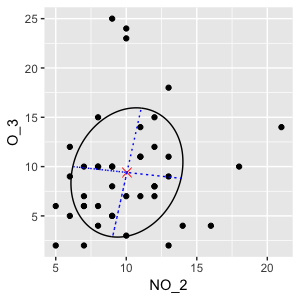
\includegraphics[width=.8\linewidth]{plot_4_29_b_ellipse.png}
  \caption{before transformation}
  \label{fig:sfig1}
\end{subfigure}%
\begin{subfigure}{.5\textwidth}
  \centering
	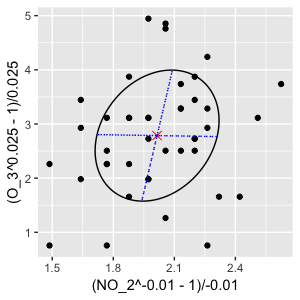
\includegraphics[width=.8\linewidth]{plot_4_29_b_ellipsenew.png}
  \caption{after transformation}
  \label{fig:sfig2}
\end{subfigure}
\caption{Confidence ellipses with bound determined by $\mathcal{X}_2^2(0.5)=1.386$}
\end{figure}

	\item[\bf{c)}] Another tool that can be used in assessing the normality of the bivariate distribution is the chi-squared plot. This plot is essentially the extension of the quantile-quantile plot to multiple dimensions. The plot is also helpful for identifying potentially outlying observations. Chi-square plots of both the untransformed and transformed data are shown in Figure 9.
\begin{figure}[H]
\begin{subfigure}{.5\textwidth}
  \centering
	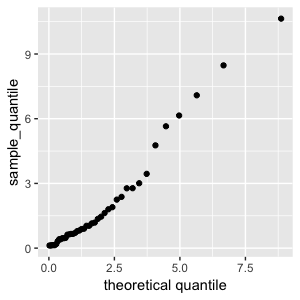
\includegraphics[width=.8\linewidth]{plot_4_29_c.png}
  \caption{before transformation}
  \label{fig:sfig1}
\end{subfigure}%
\begin{subfigure}{.5\textwidth}
  \centering
	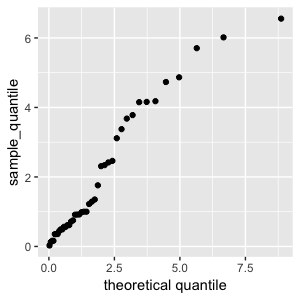
\includegraphics[width=.8\linewidth]{plot_4_29_cnew.png}
  \caption{after transformation}
  \label{fig:sfig2}
\end{subfigure}
\caption{Chi-square plots, the multivariate extension of quantile-quantile plots.}
\end{figure}

\end{enumerate}

\newpage
\section*{Problem 4.30}
This problem focuses on the used car data presented in Exercise 1.2. This is a bivariate dataset composed of ten observations. For each individual variable, as well as for the join distribution of both variables, an ideal transformation of the data is sought. For the remainder of this problem, let $X_1$ represent the age of the vehicle in years and let $X_2$ represent the selling price in thousands of US dollars

\begin{enumerate}
	\item[\bf{a)}] For $X_1$, a univariate Box-Cox method seeks the parameter, $lambda$, that maximizes the following equation: $$\max_{\lambda} l(\lambda) \equiv \max_{\lambda} \frac{-n}{2} \log{\frac{1}{n} \sum_{i=1}^n \p{x_i^{(\lambda)} - \bar{x^{(\lambda)}}}^2} + \p{\lambda - 1}\sum_{i=1}^n \log{x_i}$$ Where the transformation on $x$ is defined as: $$x^{(\lambda)} = \left\{ \begin{array}{cl} \frac{x^{\lambda} - 1}{\lambda} & if \lambda \neq 0 \\ \log{x} & if \lambda = 0 \end{array} \right.$$ The method of identifying the maximum likelihood estimator, $\hat{\lambda}$, consists of iterating through a selection of values of $\lambda$ and selecting the value which maximizes the function defined above. Graphically, this should be the apex of the curve that is formed from the empirical data. From the simulation, the maximum likelihood estimator is $\hat{\lambda}_1 = 0.37$. See Figure 10 for the associated plots.
\begin{figure}[H]
\begin{subfigure}{.33\textwidth}
  \centering
	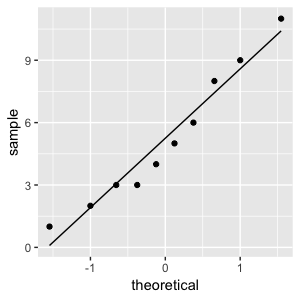
\includegraphics[width=.8\linewidth]{plot_4_30_a_qq.png}
  \caption{quantile-quantile plot before transformation}
  \label{fig:sfig1}
\end{subfigure}%
\begin{subfigure}{.33\textwidth}
  \centering
	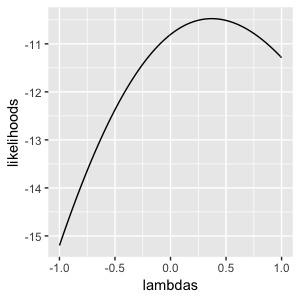
\includegraphics[width=.8\linewidth]{plot_4_30_a_bxcx.png}
  \caption{Box-Cox likelihood}
  \label{fig:sfig2}
\end{subfigure}
\begin{subfigure}{.33\textwidth}
  \centering
	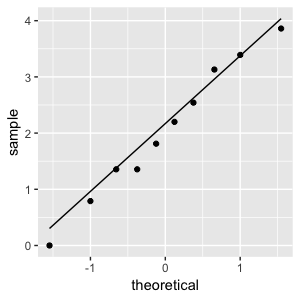
\includegraphics[width=.8\linewidth]{plot_4_30_a_qqnew.png}
  \caption{quantile-quantile plot after transformation}
  \label{fig:sfig2}
\end{subfigure}
\caption{Selected plots relating to the transformation of $X_1$.}
\end{figure}

	\item[\bf{b)}] The analysis carried out in part $\bf{a)}$ is repeated for $X_2$. The numerical analysis of the empirical data suggests that the maximum likelihood estimator for this variable is $\hat{\lambda}_2 = 0.94$. This suggests that the variable is already near the optimization point prior to transformation, i.e., the transformation is likely not necessary. The same visual analysis is presented in Figure 11.
\begin{figure}[H]
\begin{subfigure}{.33\textwidth}
  \centering
	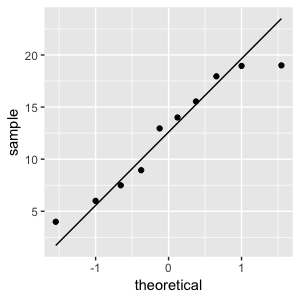
\includegraphics[width=.8\linewidth]{plot_4_30_b_qq.png}
  \caption{quantile-quantile plot before transformation}
  \label{fig:sfig1}
\end{subfigure}%
\begin{subfigure}{.33\textwidth}
  \centering
	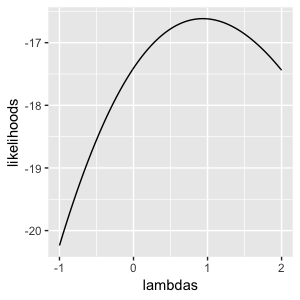
\includegraphics[width=.8\linewidth]{plot_4_30_b_bxcx.png}
  \caption{Box-Cox likelihood}
  \label{fig:sfig2}
\end{subfigure}
\begin{subfigure}{.33\textwidth}
  \centering
	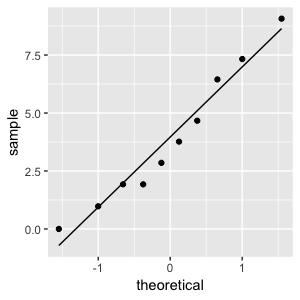
\includegraphics[width=.8\linewidth]{plot_4_30_b_qqnew.png}
  \caption{quantile-quantile plot after transformation}
  \label{fig:sfig2}
\end{subfigure}
\caption{Selected plots relating to the transformation of $X_2$.}
\end{figure}

	\item[\bf{c)}] This portion of the analysis now focuses on optimizing the bivariate transformation of $X_1$ and $X_2$. A naive approach is to simply apply the univariate transformations to each of the variables. However, this exercise will show that this is not necessarily the best approach. Because $X_1$ is highly negatively correlated with $X_2$, the behavior of the transformation is different for the joint distribution of the random variables. The method of optimization is similar, but now we seek an optimal $\vec{\lambda}$ that maximizes a combined likelihood function given by: $$\max_{\vec{\lambda}}=\frac{-n}{2} \log{det \p{\mf{S}^{(\vec{\lambda})}}} + \sum_{j=1}^p \p{\p{\lambda_j - 1} \sum_{i=1}^n \log{x_{ij}}}$$ Instead of optimizing over a vector of possible values of $\lambda$, this method optimizes over the p-dimensional array of values that defines the simulated space of $\vec{\lambda} \in \mathbb{R}^p$. For a bivariate transformation, this means that the optimal value of $\vec{\lambda}$ is attained at the maximum point of the surface shaped by the previously defined likelihood function. \\
		\\
		A likelihood function is constructed to attain such a maximization given any number of parameters. This method employs an exhaustive grid search and then selects the maximum point of the surface. The code for the function, as well as its example output that confirms its use for parts $\bf{a)}$, $\bf{b)}$, and the bivariate case are presented along with a three dimensional plot that represents the optimization surface for the bivariate case (Figure 12). This suggests that the empirical maximum likelihood estimator is $\hat{\vec{\lambda}} = \m{\hat{\lambda}_1 = 1.25 \\ \hat{\lambda}_2 = 0.05}$.
\begin{figure}[H]
\begin{subfigure}{.5\textwidth}
  \centering
	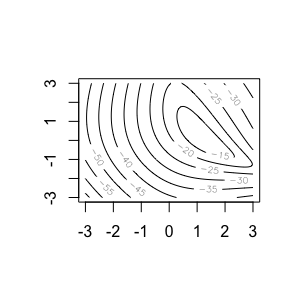
\includegraphics[width=.8\linewidth]{plot_4_30_c_contour.png}
	\caption{Contour plot of the bivariate likelihood function.}
  \label{fig:sfig1}
\end{subfigure}%
\begin{subfigure}{.5\textwidth}
  \centering
	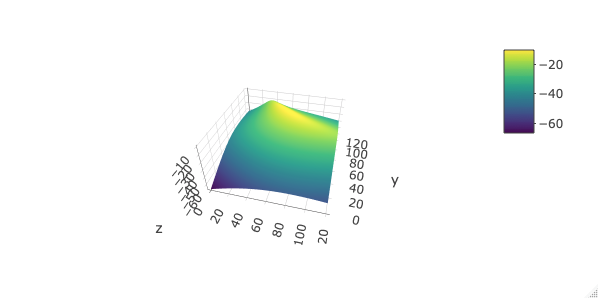
\includegraphics[width=.8\linewidth]{plot_4_30_c_manifold.png}
  \caption{Three dimensional manifold representing the optimization surface.}
  \label{fig:sfig2}
\end{subfigure}
\caption{Selected plots relating to the transformation of the joint distribution of $X_1$ and $X_2$.}
\end{figure}


\end{enumerate}

\end{document}



